Proposition~\ref{prop:escape} says that a selector fixing the retained set
before any score exists is not bound by the twofold ceiling, and that its
operation-count saving grows without limit as the retained set shrinks. That is
a statement about counts, and this paper is about what counts fail to predict.
This section instantiates the escape and measures it.

We use two selectors, both corresponding to mechanisms multi-agent
communication already uses. The first retains each agent's $k$ nearest peers by
Euclidean distance over two-dimensional positions, which is what
neighbourhood-based communication does \citep{jiang2018dgn,jiang2018atoc}. Its
selector is still pairwise, but pairwise in two dimensions rather than in the
head dimension, so it costs a factor of $d/2$ less than forming the scores. The
second orders agents along a Morton curve and retains the $k$ agents adjacent in
that order, at $O(N \log N)$, which satisfies the $o(Nkd)$ condition of
case~(i). Both then evaluate attention scores for the retained pairs only, so
the score term falls from $N^2d$ to $Nkd$ and the ceiling does not apply.

The attention over the retained peers is measured twice: once composed from
library operators, and once as a fused kernel that reads one key row and one
value row per retained peer and accumulates with a running maximum, writing
nothing but the result. Section~\ref{sec:fused} establishes that a composed
constant is an upper bound and not a property of a design, and it would be
incoherent to apply that standard to the mechanism this paper criticises and not
to the one it proposes. The two selectors attend to different peers than a
top-$k$ rule would, so what follows compares cost and not quality, and every
ratio is against the faster of the library dense kernel and our own.

\begin{table}[t]
\centering\small
\caption{Selecting before scoring, at \PrescoreK{} retained peers, every ratio
against the better of the vendor library and our own dense kernel at the tiling
the search of Section~\ref{sec:fused} found. Composing the attention stage from
library operators costs an order of magnitude more than fusing it, and the
difference decides the conclusion: composed, the attention is slower than dense
attention at every configuration measured; fused, it is up to seventeen times
faster.}
\label{tab:prescore}
\resizebox{\linewidth}{!}{\begin{tabular}{rlr rrr r rr}
\toprule
& & \textbf{ops} & \multicolumn{3}{c}{\textbf{measured (ms)}} & \textbf{best}
& \multicolumn{2}{c}{\textbf{$\div$ best dense}} \\
\cmidrule(lr){4-6}\cmidrule(lr){8-9}
$N$ & selector & saved & select & attend & total & dense & attend & total \\
\midrule
48 & nearest neighbours & 8 & 0.151 & 0.064 & 0.167 & 0.035 & 1.85 & 4.85 \\
48 & Z-order window & 10 & 0.367 & 0.059 & 0.386 & 0.035 & 1.72 & 11.18 \\
96 & nearest neighbours & 11 & 0.188 & 0.068 & 0.206 & 0.051 & 1.33 & 4.03 \\
96 & Z-order window & 20 & 0.362 & 0.065 & 0.385 & 0.051 & 1.28 & 7.53 \\
192 & nearest neighbours & 15 & 0.378 & 0.097 & 0.442 & 0.086 & 1.13 & 5.17 \\
192 & Z-order window & 39 & 0.366 & 0.095 & 0.410 & 0.086 & 1.11 & 4.79 \\
384 & nearest neighbours & 17 & 1.871 & 0.173 & 2.024 & 0.169 & 1.02 & 11.96 \\
384 & Z-order window & 78 & 0.374 & 0.171 & 0.478 & 0.169 & 1.01 & 2.82 \\
512 & nearest neighbours & 18 & 4.986 & 0.231 & 5.192 & 0.186 & 1.24 & 27.90 \\
512 & Z-order window & 104 & 0.131 & 0.221 & 0.372 & 0.186 & 1.19 & 2.00 \\
\bottomrule
\end{tabular}%
}
\end{table}

\begin{figure}[t]
\centering
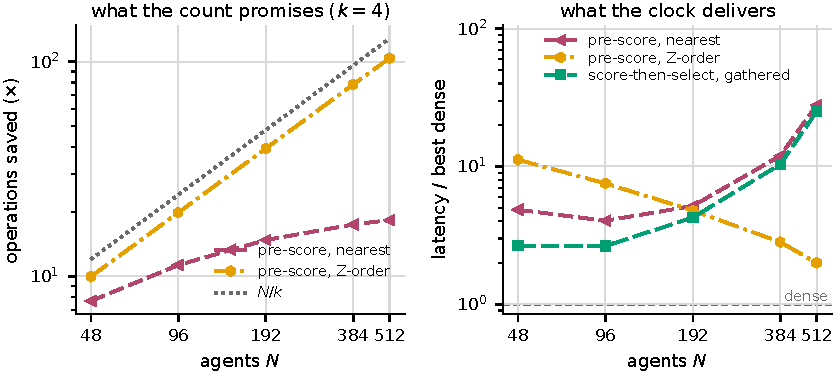
\includegraphics[width=\linewidth]{figures/fig5_prescore.pdf}
\caption{\textbf{Left:} the operation-count saving
Proposition~\ref{prop:escape} promises, which for the sub-quadratic selector
tracks $N/k$. \textbf{Middle:} what the same configurations cost. Fused, the
attention over pre-chosen peers is more than an order of magnitude faster than
dense attention at the largest agent count, and the total is then governed by
the selector, which is where the two selectors diverge. \textbf{Right:} how far
the end-to-end crossing extends. It holds at two and four retained peers, is
level with dense at eight and gone by sixteen.}
\label{fig:prescore}
\end{figure}

Fused, the escape delivers, and how much of it depends on how many peers are
kept. At two retained peers the attention stage costs $0.67$, $0.35$, $0.19$,
$0.08$ and $0.06$ times dense attention from $48$ to $512$ agents; at four,
$0.76$, $0.43$, $0.25$, $0.12$ and $0.09$. The best case over the grid is
$0.060$, nearly seventeen times faster than dense, at $512$ agents and two
retained peers. The advantage narrows as $k$ grows and at sixteen retained peers
it has gone at the smallest agent count, where the stage costs $1.26$ times
dense behind the Z-order selector and $1.58$ behind the nearest-neighbour one,
whose retained rows are scattered rather than adjacent. That shape is what Proposition~\ref{prop:escape} predicts once the score
term shrinks with the aggregation, and no score-then-select implementation
anywhere in this paper comes close to it at any sparsity, because none of them
can remove the score term.

Composed from library operators, the same stage is slower than dense attention
at every one of the forty configurations, by $1.03$ to $6.25$ times. Fusing it
is worth between $3.9$ and $17.4$ times, and the factor grows with the agent
count because the gathered tensor the composition writes and re-reads grows with
it. We report both columns because the composed one is what we measured before
writing the kernel, and on its own it supports the opposite conclusion.

What decides the total is the selector, and the two behave oppositely. The
Z-order selector's cost is nearly flat in the agent count --- $0.096$ to
$0.140$\,ms across the range --- so as attention grows more expensive the
selector's share of the path falls: at four retained peers the whole path costs
$16.8$, $8.8$, $4.0$, $1.28$ and $0.91$ times dense attention from $48$ to $512$
agents. At $512$ agents, selecting before scoring and executing both stages in
kernels written for them is about ten per cent faster end to end than the best
dense attention we can obtain, and the trend is still improving. That crossing
is the whole of it: it holds at two and at four retained peers, the path is
level with dense at eight ($1.01$) and behind it at sixteen ($1.17$), and at
$384$ agents it is behind at every sparsity. Both runs of the sweep put the
crossing cells within one and a half per cent of each other, so the margin is
small but not noise. The nearest-neighbour selector moves the other way. It
materialises an $N \times N$ distance matrix and ranks it --- the same two
operations, on the same shape, that Proposition~\ref{prop:ceiling} says a
score-then-select rule cannot avoid --- so beyond $96$ agents its cost grows
quadratically and the path it belongs to rises to $30.8$ times dense, with the
fused attention stage making no difference to that outcome.

Three things follow, and together they are the paper's constructive result.

Escaping the operation-count ceiling is necessary and not sufficient. Both
selectors escape it, by between $7$ and $107$ times in operations at
four retained peers, and one of
them is an order of magnitude slower than dense attention while the other is
faster. What separates them is whether the selector reaches its decision through
a structure of the size it was introduced to avoid.
Proposition~\ref{prop:escape} charges for the selector in operations, and
operations are the wrong currency: the nearest-neighbour selector's arithmetic
is small and its traffic is exactly the traffic the ceiling is about.

A cheap selector is not sufficient either. With the attention stage composed
from library operators the Z-order path is slower than dense at every agent
count we measure, and only the fused kernel makes the total cross. Both
conditions are needed, and an operation count expresses neither.

And the regime matters. The crossover arrives at a few hundred agents and
improves beyond it, which is above the range most of the multi-agent
communication literature occupies (Section~\ref{sec:related}) and far below the
range where block-sparse attention operates. Whether a method between the two
should sparsify its communication is now a question with a checkable answer
rather than an appeal to an operation count: it depends on whether the selector
avoids a quadratic intermediate, and on whether the sparse attention it leaves
behind is executed in a kernel written for it.
